\section{黑体辐射}

\begin{quotation}
``......重要的是用一种尽可能保守的方式来进行工作,就是说,只有那些已被证明为绝对必要的变化才应该被引入到现存的理论中。''\qquad 普朗克
\end{quotation}

\subsection{预备知识}

\index{Thermal radiation: 热辐射}

热辐射是热量传递方式之一。物体之间的空间存在辐射场,
辐射场是各种频率的电磁波在空间的分布。
物体可通过发射、吸收电磁波的过程与其周围的辐射场交换能量。
辐射场可看作是光子气,即把辐射场看作是许多不同频率,
但全部以光速$c$运动彼此完全独立的光子体系 \footnote{参考:M. W.
泽门斯基, R. H. 迪特曼, {\bf 热学和热力学}, p511;}。
我们一般考虑处在热平衡状态下的物体与辐射场,它们有相同的温度$T$。

为定量描述辐射场,及辐射场与物体间的能量交换,引入:辐射场能量的分布函数:
$f(\nu ,\hat k,r,t)d\nu d\Omega$,

其中: $\hat k$
代表光子传播方向单位矢量,r是空间位置矢量,t是时间。如果辐射场是均匀的,则f与r无关,
如辐射场是恒定的,则f与t无关,如辐射场是各向同性的,则f与$\hat k$无关。

定义1:辐射场能量的谱密度$u(\nu )$:

\begin{equation*}
u(\nu ,r,t) = \int {f(\nu ,\hat k,r,t)d\Omega }  = \int_0^{2\pi }
{d\varphi \int_0^\pi  {d\theta \sin \theta f(\nu ,\theta ,\varphi
,r,t)} }
\end{equation*}

假设辐射场是各向同性的,则:

\begin{equation}
u(\nu ,r,t) = 4\pi f(\nu ,r,t)
\end{equation}

定义2:辐射通量谱密度$\Delta j(\nu )$:

\begin{eqnarray*}
\Delta j(\nu ,r,t) & =  & \int\limits_{2\pi } {cf(\nu ,\hat k,r,t)\hat k
\cdot \Delta S d\Omega }  \\
{} & = & \int_0^{2\pi } {d\varphi
\int_0^{{\raise0.5ex\hbox{$\scriptstyle \pi $}
\kern-0.1em/\kern-0.15em \lower0.25ex\hbox{$\scriptstyle 2$}}}
{d\theta \sin \theta \cos \theta  \cdot cf(\nu ,\theta ,\varphi
,r,t)} }
\end{eqnarray*}

假设辐射场是各向同性的,$\Delta S$是单位面元矢量,$\hat k \cdot
\Delta S = \cos \theta $,则:

\begin{equation}
\Delta j(\nu ,r,t) = \pi cf(\nu,r,t)\Delta S
\end{equation}

\begin{figure}[h]
\begin{center}
  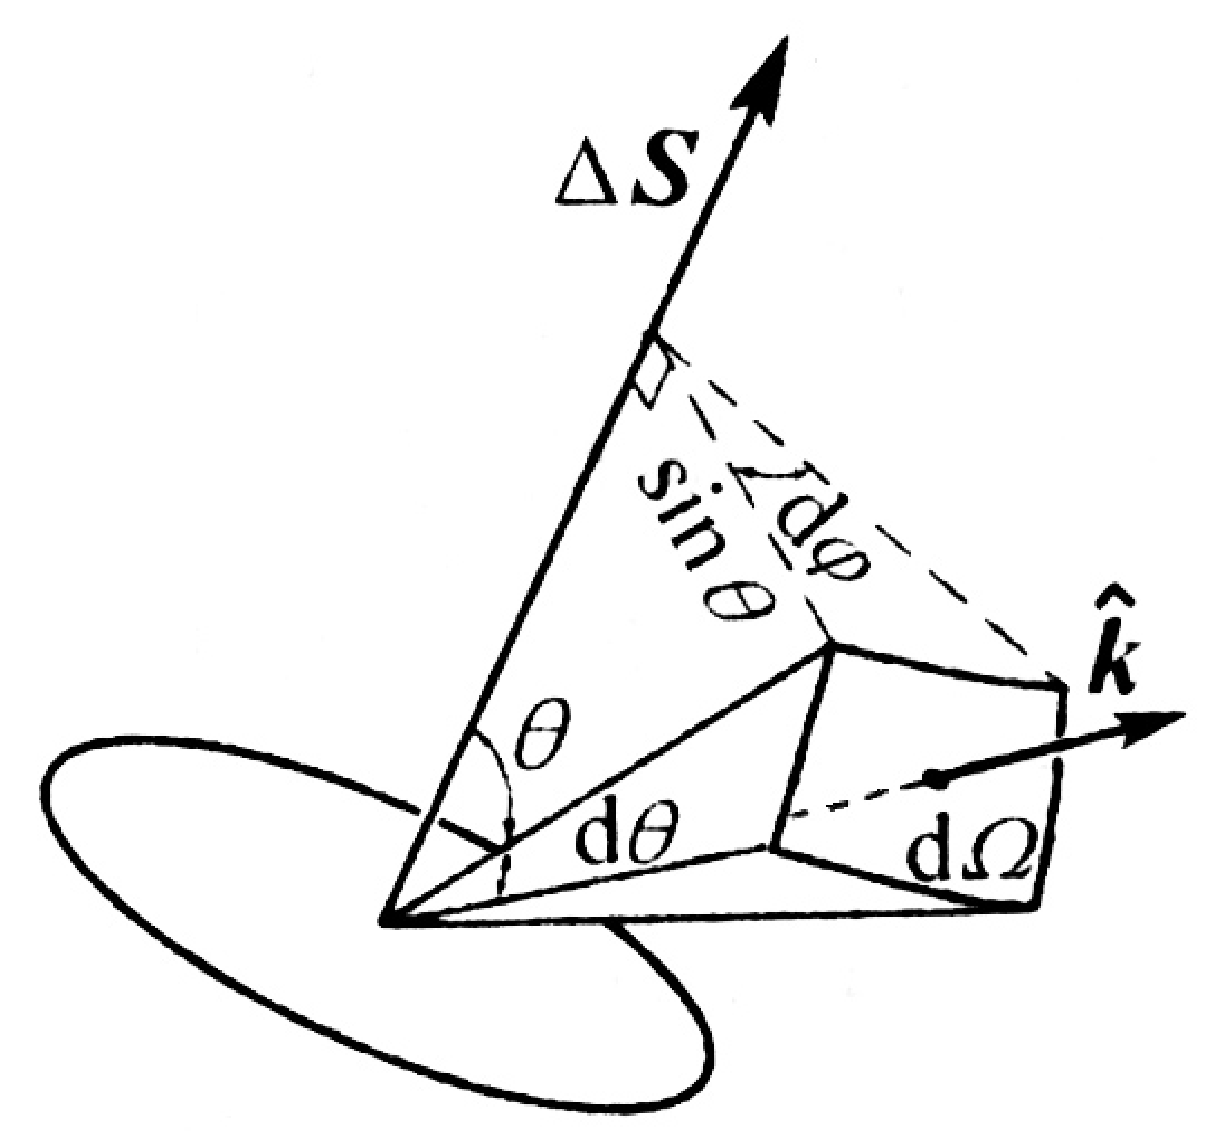
\includegraphics[width=5cm]{Duality/2-1.ps}\\
  \caption{球坐标表示立体角}\label{2-1}
\end{center}
\end{figure}

上式中的$c$是电磁辐射能流的速率(即光速),对立体角的积分限于面元$\Delta S$的一侧($2\pi$)。积分时取以面元法线$\Delta S$为极轴的球坐标系,用$\theta$、$\varphi$来表示传播方向$\hat k$。


定义如下辐射场与物体间交换能量的物理量:
\begin{enumerate}
    \item 辐射本领(物体表面单位面积发出的辐射通量)谱密度:$r(\nu ) = \frac{{dj(\nu )}}{{dS}}$
    \item 辐射照度(照射在物体表面单位面积上的辐射通量)谱密度:$e(\nu ) = \frac{{dj'(\nu )}}{{dS}} = \pi cf = \frac{c}{4}u(\nu )$
    \item 吸收本领:$\alpha (\nu ) = \frac{{dj''(\nu )}}{{dj'(\nu )}}$,即吸收的辐射通量密度与照射的辐射通量密度之比,显然此比值在0,1之间。
\end{enumerate}

\index{Kirchhoff's law: 基尔霍夫定律}

基尔霍夫热辐射定律(Kirchhoff's
law):在热平衡状态下的辐射场,应是均匀、恒定、各向同性的,其能谱密度$u_T
(\nu )$ 应仅与平衡时温度T,和$\nu $有关,即$u_T (\nu
)$是一个与物质无关的普适函数,称为:热辐射的标准能谱。

在平衡态下,任一表面积上发出的能量$r(\nu ,T)$与吸收的能量$\alpha (\nu )\frac{{dj'}}{{dS}} = \alpha (\nu )e(\nu ,T)$
相等。即:$r(\nu ,T) = \alpha (\nu )e(\nu ,T)$。

所以:

\begin{equation}
\frac{{r(\nu ,T)}}{{\alpha (\nu )}} = e(\nu ,T) = \frac{c}{4}u_T (\nu )
\end{equation}

即:辐射本领与吸收本领成正比,比值只与$\nu $和T有关。

\subsection{黑体辐射}

绝对黑体:物体的吸收本领$\alpha (\nu
,T)$与$\nu$和T无关,恒等于1,简称黑体。 即绝对黑体辐射本领:$r_b
(\nu ,T) = \frac{c}{4}u_T (\nu )$,
所以只要测量绝对黑体的辐射本领,即可获得热辐射的标准能谱。

\index{Black body: 黑体}

和质点一样,黑体是理想的物理模型,实际物质不可能是真正的黑体。我们一般用开有小孔,内壁粗糙的空腔来表示它。光射进小孔后,要经过内壁无穷次反射后,才有非常微弱的光从小孔重新射出,孔越小,从小孔处反射出的光越微弱,近似可看作光全部被吸收。用这种方法人们可以制备非常理想的黑体,并测量黑体辐射谱。

\begin{figure}[h]
\begin{center}
  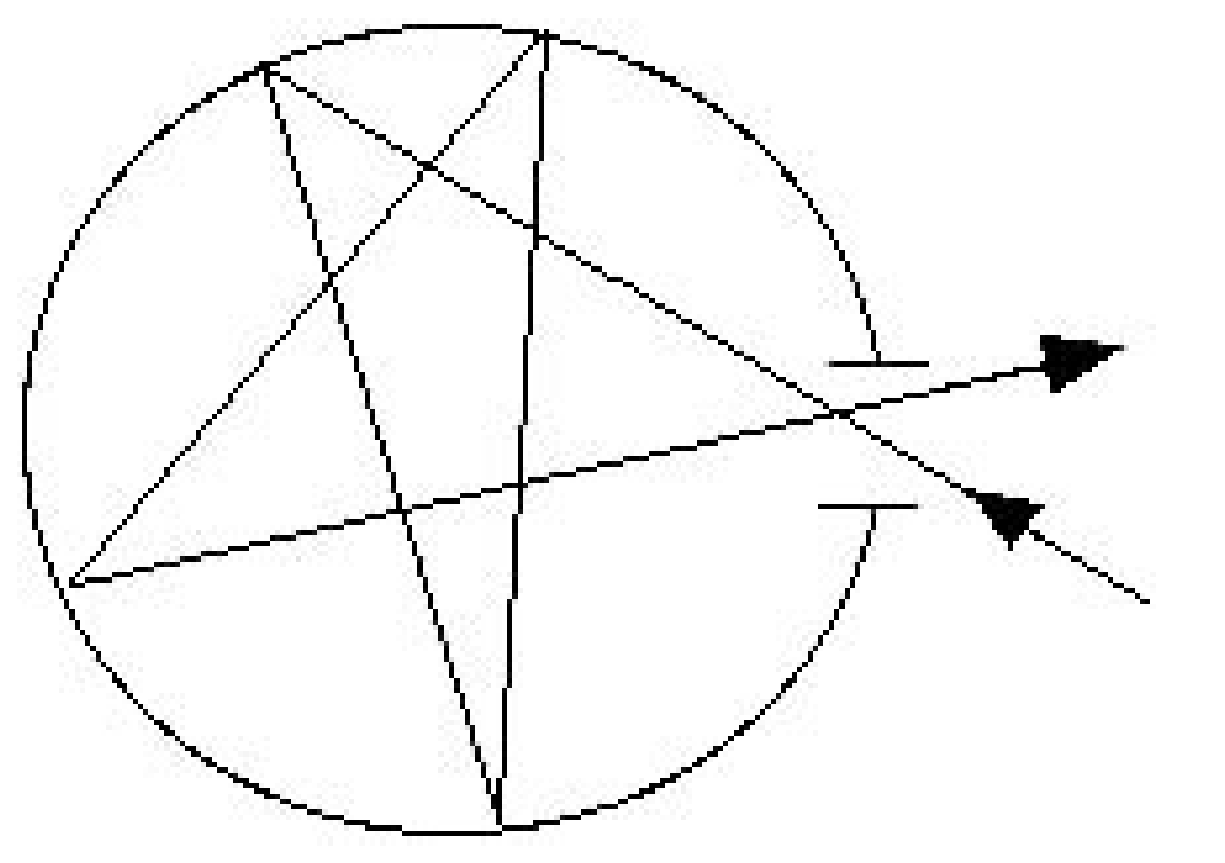
\includegraphics[width=5cm]{Duality/2-2.ps}\\
  \caption{绝对黑体的制备}\label{blackbody}
\end{center}
\end{figure}

需要注意的是,这里的黑体是小孔,而非空腔。这种黑体对我们来说并不陌生,典型的例子就是炼钢的高炉,或动画片《大闹天宫》中太上老君炼丹的炉子。对空腔(炼丹炉)加热,我们可测量由小孔(黑体)辐射出的不同温度下的热辐射曲线。

\begin{figure}[h]
\begin{center}
  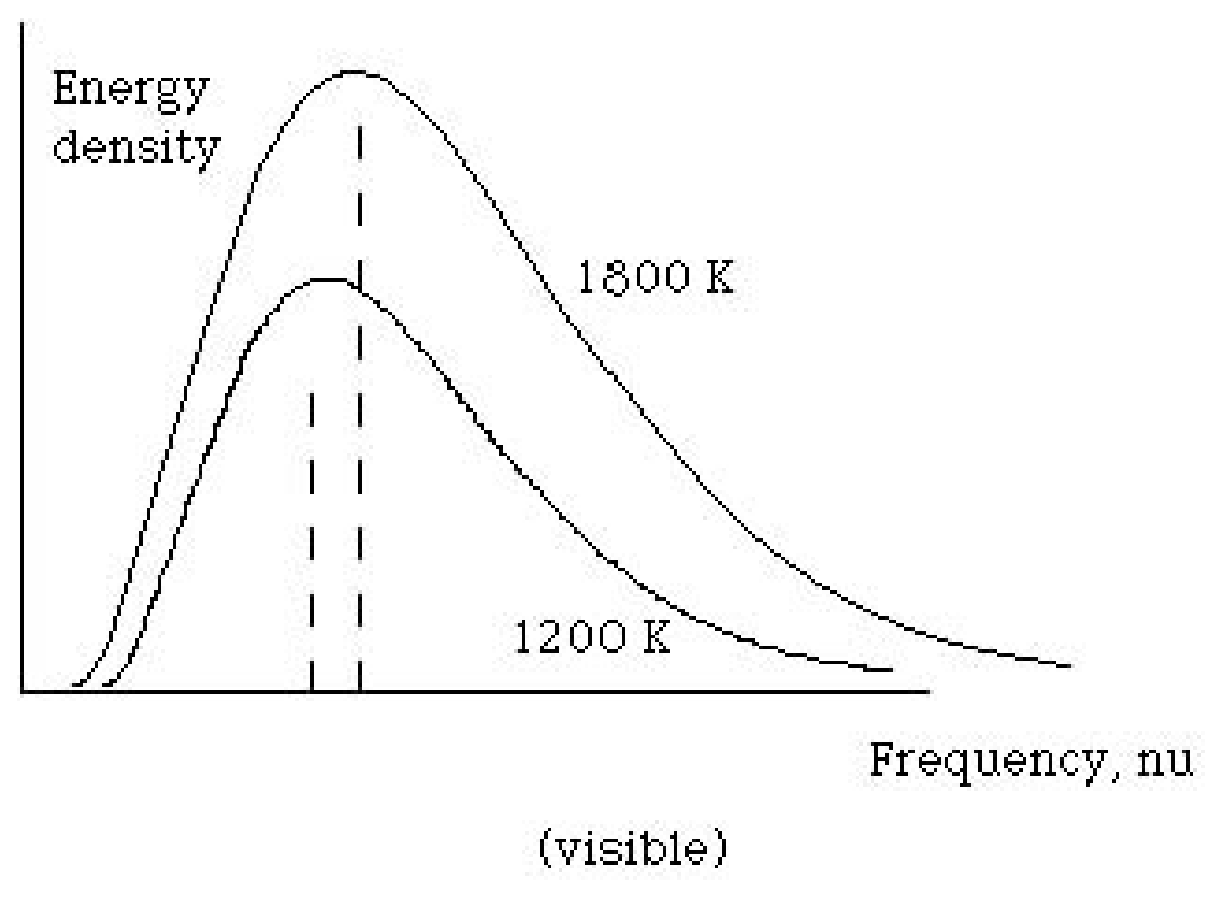
\includegraphics[width=6cm]{Duality/2-3.ps}\\
  \caption{不同温度下的黑体辐射谱}\label{blackbody radiation}
\end{center}
\end{figure}

实验满足以下规律:

\index{Wien's displacement law: 维恩位移定律}

\index{Stefan and Boltzman's law: 斯特番-玻耳兹曼定律}

\begin{enumerate}
    \item {维恩位移定律(Wien's displacement law):$\lambda _{\max } T = 2.898 \times 10^{-3} m K$,即随着温度升高,热辐射峰值向短波高频方向移动。

当孙悟空进入太上老君的炼丹炉的时候,老君通过观察炉口的颜色来判断炉子的温度,刚开始的时候是红色的,然后就是“黄绿青蓝紫”,波长越来越短,炉子的温度越来越高。}

    \item {斯特番-玻耳兹曼定律(Stefan and Boltzman's law):黑体辐射本领$R(T) = \int_0^\infty  {r_b (\lambda ,T)d\lambda } $与热力学温度四次方成正比,即:$R(T) = \sigma T^4 $, $\sigma  = 5.67 \times 10^{ - 8} Js^{ - 1} m^{ - 2} K^{ - 4} $
叫作斯特番-玻耳兹曼常数。}

    \item {为了解释黑体辐射的实验数据,维恩假设气体分子辐射频率只与其速度有关,得到维恩公式:$u_T (\nu ) = \frac{{\alpha \nu ^3 }}{{c^2 }}e^{ - {\raise0.7ex\hbox{${\beta \nu }$} \!\mathord{\left/
 {\vphantom {{\beta \nu } T}}\right.\kern-\nulldelimiterspace}
\!\lower0.7ex\hbox{$T$}}} $,其中:$\alpha$,$\beta$为常量。}

    \item {瑞利根据能量按自由度均分和经典电动力学,得到瑞利-金斯公式(Rayleigh and Jeans law):$u_T (\nu ) = \frac{{8\pi }}{{c^3 }}\nu ^2 k_B T$,显然这个公式对高频无效,因为此时能量密度趋于无限大,这就是著名的紫外灾难。}
\end{enumerate}

\index{Wien's Formula: 维恩公式}

\index{Rayleigh and Jeans law: 瑞利-金斯公式}

\index{Ultraviolet disaster: 紫外灾难}

\begin{figure}[h]
\begin{center}
  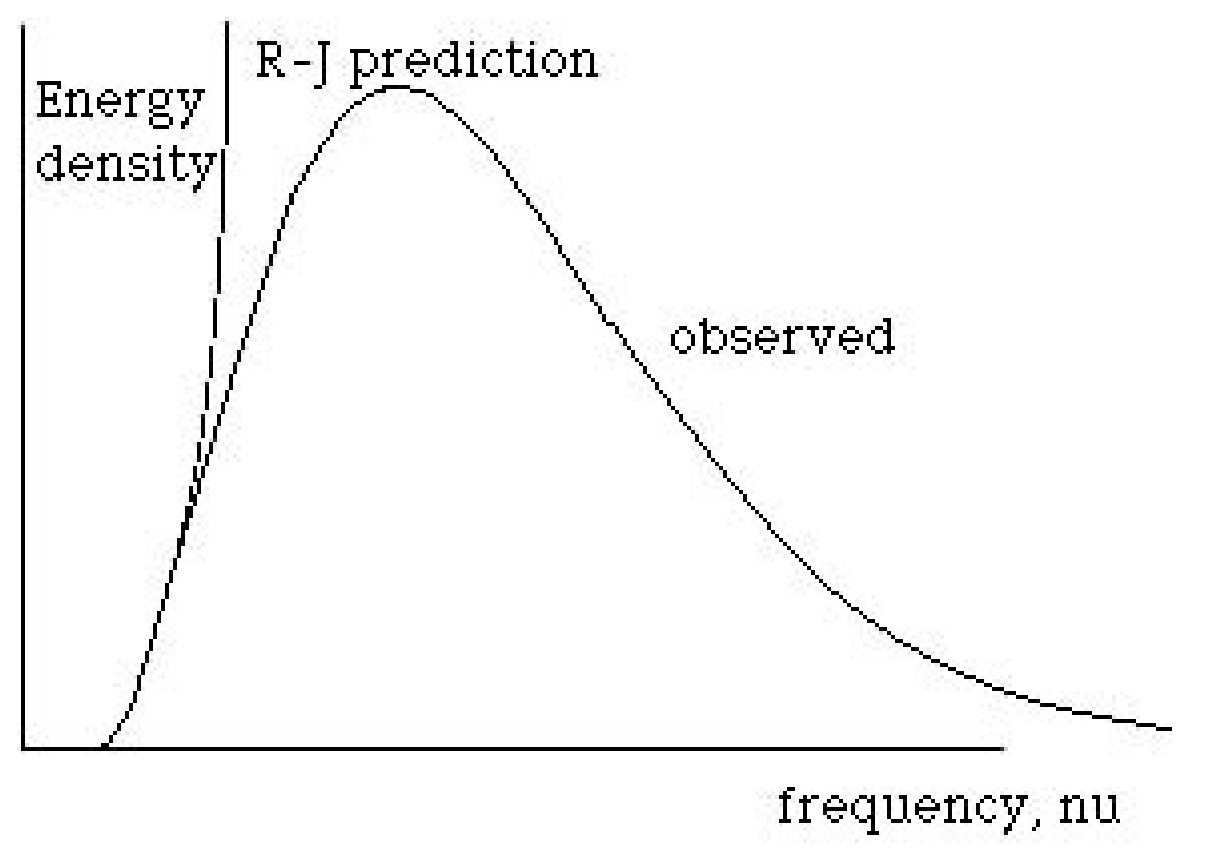
\includegraphics[width=6cm]{Duality/2-4.ps}\\
  \caption{紫外灾难}\label{Rayleigh & Jeans law}
\end{center}
\end{figure}

\subsection{普朗克公式}

\begin{figure}[h]
\begin{center}
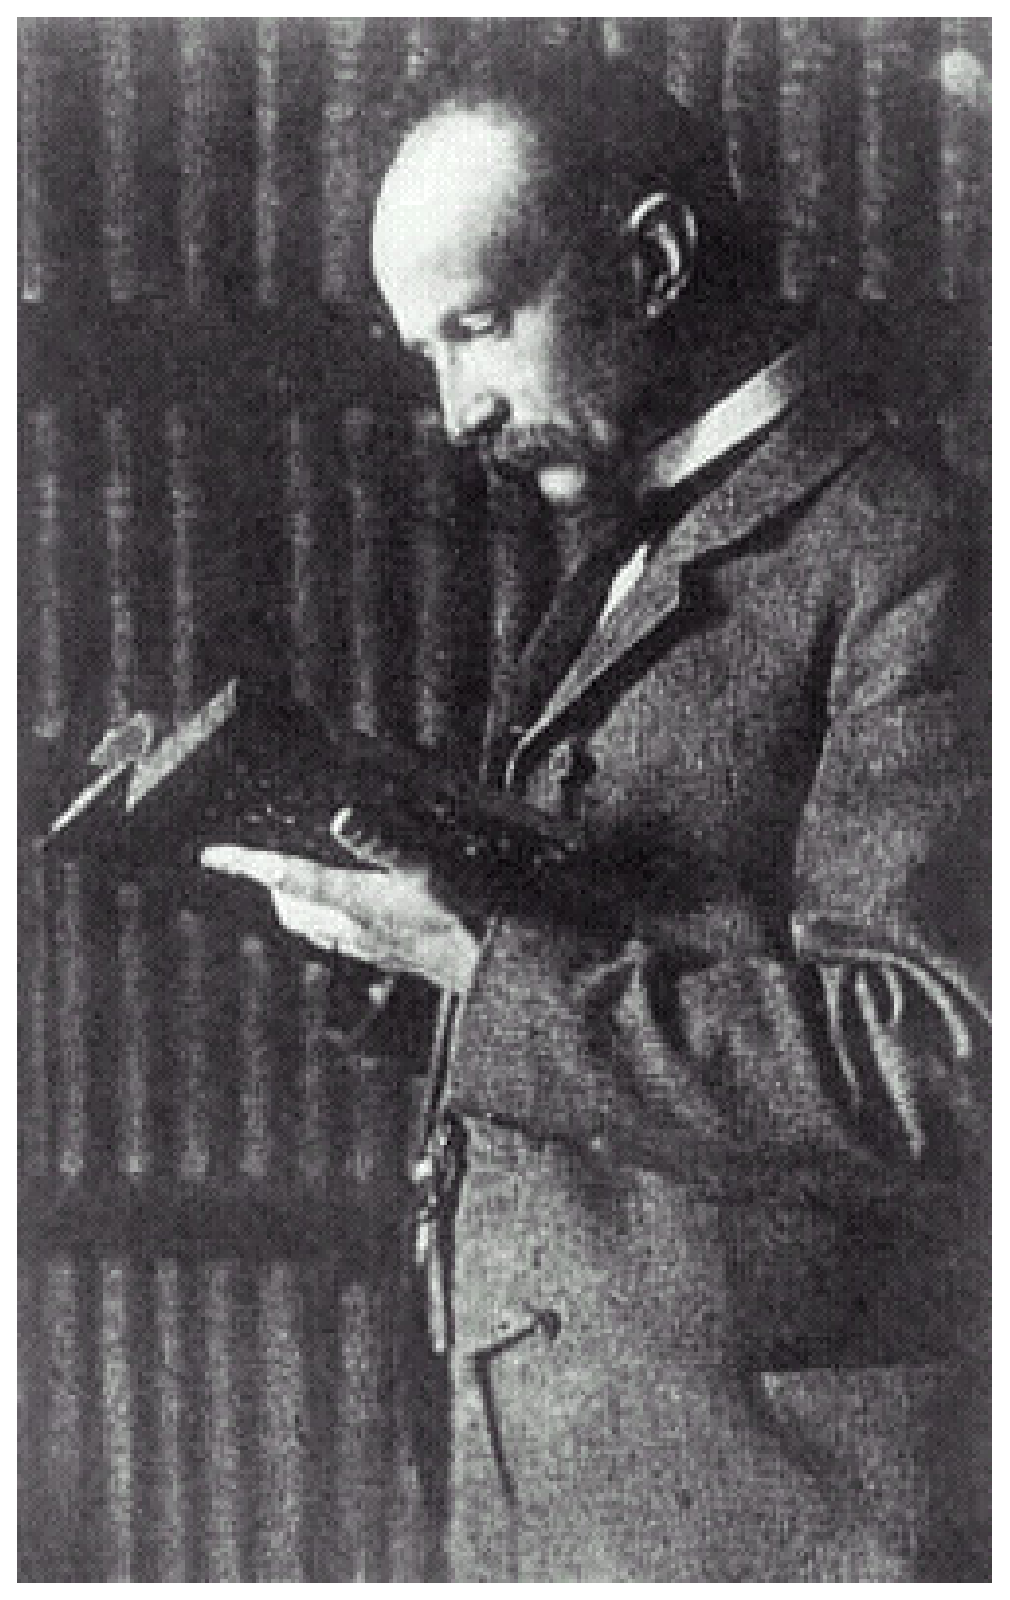
\includegraphics[width=5cm]{Duality/planck.ps}
\caption{普朗克}
\end{center}
\end{figure}

1900年,普朗克(Max Planck)使用内插法,在维恩公式和瑞利-金斯公式的基础上得到了一个新的黑体辐射能量密度公式:

\index{Planck's formula: 普朗克公式}

\begin{equation}\label{planck's law}
u_T (\nu ) = \frac{{8\pi h\nu ^3 }}{{c^3 }} \cdot \frac{1}{{e^{\frac{{h\nu }}{{k_B T}}}  - 1}}
\end{equation}

普朗克公式在整个频率范围与实验结果符合的很好,而维恩公式和瑞利-金斯公式则分别仅在高频和低频下才符合较好。

普朗克并不满足于一个经验公式,很快他得到了公式的理论解释,并提出了量子假说。
即:电磁辐射的能量只能是量子化的,$\varepsilon  = nh\nu $,$n=1,2,3...$,

\begin{equation}
h = 6.626 \times 10^{ - 34} J \cdot s
\end{equation}

$h$被称为普朗克常数,它的单位是“焦耳$\cdot$秒”。对原子物理来说,把它表示为以“电子伏$\cdot$秒”为单位将会更方便,经过简单的计算,或直接查询“WolframAlpha”得到:

\begin{equation}
h = 4.135668 \times 10^{-15} eV \cdot s
\end{equation}

\subsubsection{普朗克公式的推导}

考虑边长为L的立方体,体积内既无电荷也无电流,且有能完全反射的内表面(理想导体),也称为空腔辐射。

回忆电磁波在矩形谐振腔内的电磁振荡\footnote{参考:郭硕鸿《电动力学》,第161页。}。取导体壁的内表面分别为$x=0$和$x=L$,
$y=0$和$y=L$,$z=0$和$z=L$。空腔内电磁波的电场和磁场任一直角分量都满足亥姆霍兹方程:

\begin{equation}
\left( {\nabla ^2  + k^2 } \right)\left\{ {\begin{array}{*{20}c}
   {\mathord{\buildrel{\lower3pt\hbox{$\scriptscriptstyle\rightharpoonup$}}
\over E} }  \\
   {\mathord{\buildrel{\lower3pt\hbox{$\scriptscriptstyle\rightharpoonup$}}
\over B} }  \\
\end{array}} \right\} = 0
\end{equation}

利用分离变量法, 可解出电场分量为:

\index{Separation of variables: 分离变量}

\begin{equation}
\left\{ \begin{array}{l}
 E_x  = A_1 \cos k_x x\sin k_y y\sin k_z z \\
 E_y  = A_2 \sin k_x x\cos k_y y\sin k_z z \\
 E_z  = A_3 \sin k_x x\sin k_y y\cos k_z z \\
 \end{array} \right.
\end{equation}

其中:$k_x  = \frac{{n_x \pi }}{L},k_y  = \frac{{n_y \pi }}{L},k_z =
\frac{{n_z \pi }}{L}$, $n_x ,n_y ,n_z  = 0,1,2,3,...$ ($n_x ,n_y
,n_z$中至少要有两个不为0,否则电场$\hat E = 0$)。

由于立方体内没有电荷分布,$\nabla \cdot \hat E =0$,所以:

\begin{equation}
k_x A_1 + k_y A_2 + k_z A_3 = 0
\end{equation}

因此$A_1$,$A_2$,和$A_3$中有两个是独立的,即对每一组 $(n_x, n_y,
n_z)$ 的本征振荡,有两个独立的偏振模。

考虑波矢空间($\vec k$空间):

\begin{equation}
k^2  = k_x ^2  + k_y ^2  + k_z ^2  = \left( {\frac{\pi }{L}} \right)^2 \left( {n_x ^2  + n_y ^2  + n_z ^2 } \right)
\end{equation}

空腔辐射可能状态(满足驻波条件的状态)坐落在$\left( {\frac{\pi }{L}} \right)$
间距的一系列格点上,即每个状态占据$\left( {\frac{\pi }{L}} \right)^3 $相空间体积。所以$k$半径内总状态数为:

\begin{equation}
N(k) = \frac{1}{8} \cdot \frac{{4\pi k^3 }}{3} \cdot 2 \cdot \left( {\frac{L}{\pi }} \right)^3 = \frac{{\pi k^3 }}{3} \cdot \left( {\frac{L}{\pi }} \right)^3 
\end{equation}

其中:1/8是由于积分仅对第一卦限进行,2是由于每一组$(n_x, n_y, n_z)$的本征振荡,对应两个独立的偏振模。

利用:$k = \frac{{2\pi }}{\lambda } = \frac{{2\pi \nu }}{c}$,得到:

\begin{equation}
N(\nu ) = \frac{{8\pi \nu ^3 L^3 }}{{3c^3 }}
\end{equation}

态密度(Density of states,定义为每单位能量或频率里态的数量)为:

\begin{equation}
g(\nu ) = \frac{1}{V}\frac{{dN(\nu )}}{{d\nu }} = \frac{1}{{L^3 }}\frac{{8\pi \nu ^2 L^3 }}{{c^3 }} = \frac{{8\pi \nu ^2 }}{{c^3 }}
\end{equation}

能量密度为:

\begin{equation}
u_T (\nu ) = g(\nu )\left\langle {\varepsilon (\nu ,T)} \right\rangle
\end{equation}

尖括号表示求热力学平均。

\subsubsection*{对公式的讨论}

\begin{enumerate}
    \item 按照能量均分定理,取$\left\langle {\varepsilon (\nu ,T)} \right\rangle  = k_B T$
(每个自由度均分能量$\frac{{k_B T}}{2}$,电磁场能量密度:$w = \frac{{\varepsilon _0 }}{2}E^2  + \frac{{B^2 }}{{2\mu _0 }}$ ,总平均能量为$k_B T$),于是则得到瑞利-金斯公式:

\begin{equation}\label{rayleigh}
    u_T (\nu ) = \frac{{8\pi }}{{c^3 }}\nu ^2 k_B T
\end{equation}

以上关于瑞利-金斯公式的推导是严格的,紫外灾难不可避免。
这说明在经典物理学的内部(电动力学和统计力学)蕴藏着深刻的矛盾。

(直接计算也可得到:$\left\langle {\varepsilon (\nu ,T)} \right\rangle  = \frac{{\int_0^\infty  {\varepsilon e^{ - {\raise0.7ex\hbox{$\varepsilon $} \!\mathord{\left/
 {\vphantom {\varepsilon  {kT}}}\right.\kern-\nulldelimiterspace}
\!\lower0.7ex\hbox{${kT}$}}} } d\varepsilon }}{{\int_0^\infty  {e^{ - {\raise0.7ex\hbox{$\varepsilon $} \!\mathord{\left/
 {\vphantom {\varepsilon  {kT}}}\right.\kern-\nulldelimiterspace}
\!\lower0.7ex\hbox{${kT}$}}} d\varepsilon } }} = k_B T$
)

\item 利用普朗克量子假说:电磁辐射能量$\varepsilon_n = n h \nu$,$n=0,1,2,3$,…,

\begin{eqnarray*}
\left\langle {\varepsilon (\nu ,T)} \right\rangle &=& \frac{{\sum\limits_n {\varepsilon _n e^{ - {\raise0.7ex\hbox{${\varepsilon _n }$} \!\mathord{\left/
 {\vphantom {{\varepsilon _n } {k_B T}}}\right.\kern-\nulldelimiterspace}
\!\lower0.7ex\hbox{${k_B T}$}}} } }}{{\sum\limits_n {e^{ - {\raise0.7ex\hbox{${\varepsilon _n }$} \!\mathord{\left/
 {\vphantom {{\varepsilon _n } {k_B T}}}\right.\kern-\nulldelimiterspace}
\!\lower0.7ex\hbox{${ k_B T}$}}} } }} = \frac{{\sum\limits_n {nh\nu e^{
- \beta nh\nu } } }}{{\sum\limits_n {e^{ - \beta nh\nu } } }} \\
{} &=& - \left[ {\frac{\partial }{{\partial \beta }}\ln \left( {\sum\nolimits_0^\infty  {e^{ - \beta nh\nu } } } \right)} \right] \\
{} &=& - \left[ {\frac{\partial }{{\partial \beta }}\ln \left( {\frac{1}{{1 - e^{ - \beta h\nu } }}} \right)} \right] \\
{} &= & \frac{\partial
}{{\partial \beta }}\ln \left( {1 - e^{ - \beta h\nu } } \right)
\end{eqnarray*}

这里:$\beta  = \frac{1}{{k_B T}}$,所以:

\begin{equation}
\left\langle {\varepsilon (\nu ,T)} \right\rangle  = \frac{{h\nu e^{ - \beta h\nu } }}{{1 - e^{ - \beta h\nu } }} = \frac{{h\nu }}{{e^{\beta h\nu }  - 1}}
\end{equation}

即得到普朗克公式:

\begin{equation}
u_T (\nu ) = \frac{{8\pi h\nu ^3 }}{{c^3 }} \cdot \frac{1}{{e^{\frac{{h\nu }}{{k_B T}}}  - 1}}\end{equation}

可见,为解释黑体辐射,人们必须引入能量量子化概念:频率为$\nu$的电磁辐射,其能量只能取能量子$h\nu $
的整数倍。这显然与经典物理学矛盾,按经典物理学,能量与振幅的平方成正比,可取从0到无穷大任意值
(对应于维恩公式,但有紫外发散困难)。为了解释自己的公式,普朗克假设能量量子化是由于辐射电磁波的谐振子的能量是量子化的,
电磁辐射场本身的能量是连续的,但它们之间发生能量交换时必须一份、一份地进行,即是量子化的。这种解释看起来有些牵强,
但为了避免“推翻”整个经典物理学体系,也是必然的选择。但后来,光电效应等更多实验表明,辐射场本身也是量子化的。

\index{photon: 光子}

如果我们把$h\nu $理解为光子,
则频率为$\nu$的电磁辐射,对应n个频率为$\nu$ 的光子,
即光强是由光子数目决定的,
辐射场能量分布函数$f$可以看为光子气的密度分布函数$n$。这里我们可以回忆(比较)一下分子运动论中的麦克斯韦速率分布函数:

\begin{equation}
f(v)
= 4\pi \left( {\frac{m}{{2\pi k_B T}}} \right)^{3/2}  \cdot v^2 e^{
- mv^2 /2k_B T} 
\end{equation}

\end{enumerate}

\subsection*{物理常数}

\begin{itemize}
  \item 普朗克常数:$h = 6.626 \times 10^{ - 34} J \cdot s$
  \item 维恩常数:$b = 2.898 \times 10^{-3} m \cdot K$
  \item 斯特番-玻耳兹曼常数:$\sigma  = 5.67 \times 10^{ - 8} Js^{ - 1} m^{ - 2} K^{ - 4}$
  \item 玻尔兹曼常数: $k_B =1.38 \times 10^{-23} J \cdot K^{-1}$
\end{itemize}


\subsection*{阅读与思考}

\begin{itemize}
\item 阅读《天体物理学》(李宗伟等著,高等教育出版社)第2章,``天体物理中的辐射过程'',并写出读书报告。

\item
假设太阳、地球、火星、金星都可看作是绝对黑体,
利用斯特藩-玻尔兹曼定律, 估算金星、地球和火星的表面温度,
这给出了一个讨论温室效应的定量框架。

太阳半径: $R_S  = 6.96 \times 10^5 km$;太阳表面温度: $T_S  = 5780K$;$\sigma  = 5.67 \times 10^{ - 8} Js^{ - 1} m^{ - 2} K^{ - 4} $;水星距离太阳的距离是0.39AU, 火星距离太阳的距离是1.52AU ($1AU = 1.496 \times 10^8 km$)。


解: 太阳总辐射功率: $P = \sigma T^4 4 \pi R_S^2$,
其中只有一部分会照在``地球''上, 比例是: $\frac{\pi R_E^2}{4 \pi
D^2}= \frac{R_E^2}{4 D^2}$, 这里$D$是地球距离太阳的距离(地心到日心).

假设地球表面温度是$T_E$, 地球向外辐射的功率是: $\sigma T_E^4 4 \pi
R_E^2$, 当这个辐射功率和吸收功率相等时, 可估算出地球表面的温度。

\begin{equation*}
\sigma T^4 4 \pi R_S^2 \cdot \frac{R_E^2}{4 D^2} = \sigma T_E^4 4
\pi R_E^2
\end{equation*}

解出:

\begin{equation*}
T_E = T \sqrt{\frac{R_S}{2D}} = 278.77 K
\end{equation*}

这个温度与地球半径($R_E$)无关. 更多结果见下表:

\begin{center}
\begin{tabular}{|l|l|l|l|l|}
  \hline
  % after \\: \hline or \cline{col1-col2} \cline{col3-col4} ...
  {} & 水星 & 金星 & 地球 & 火星 \\
  距离(AU) & 0.39 & 0.73 & 1 & 1.52 \\
  温度(K) & 446 & 326 & 279 & 226 \\
  温度(${}^oC$) & 173 & 53 & 6 & -47 \\
  \hline
\end{tabular}
\end{center}



\textbf{参考}:

\url{http://en.wikipedia.org/wiki/Black_body}


``Engineering the climate'',
\url{http://physicsworld.com/cws/article/print/40222}



``全球变暖之定时炸弹'', 《科学美国人》中文版, 2004年第5期, pp44-53。


\end{itemize}


\subsection*{练习}


\begin{enumerate}

\item 由黑体辐射公式导出维恩位移定律:能量密度极大值所对应的波长$\lambda_m$与温度$T$成反比,即:$\lambda_m T = B$,$B$是一常量,近似计算$B$的数值。

解: 由频率的分布$\int u_T(\nu) d\nu$出发:

\begin{equation*}
\int u_T(\nu)d\nu =\int  \frac{8\pi h
\nu^3}{c^3}\frac{1}{e^{\frac{h\nu}{k_B T}} -1} d \nu
\end{equation*}

变量变换, 把$\nu \to \lambda$, $\lambda = \frac{c}{\nu}$, $d \lambda
= - \frac{c}{\nu^2} d \nu$. 或:$\nu = \frac{c}{\lambda}$, $d\nu = -
\frac{\nu^2}{c} d\lambda=-\frac{c}{\lambda^2}d\lambda$.


\begin{equation*}
\int u_T(\nu) d \nu = \int \frac{8\pi
hc}{\lambda^5}\frac{1}{e^{\frac{hc}{k_B T\lambda}}-1} d\lambda
\end{equation*}

上式中我们把负号``-''略去不写. 现在对新的$\int u_T(\lambda)
d\lambda$中的$u_T(\lambda)$求微分. 极值条件:

\begin{equation*}
\left. {\frac{d u_T(\lambda)}{d\lambda}} \right|_{\lambda =
\lambda_{max}} = 0
\end{equation*}

令: $x = \frac{hc}{k_B T \lambda}$, 上式化简可得:

\begin{equation*}
(5-x)e^x =5
\end{equation*}

这个方程可通过``作图法''求解\footnote{Mathematica:
``FindRoot[5*Exp[x]-x*Exp[x] ==5 , \{x,10\}]''

``解析解'', 网址:

\url{http://www.udel.edu/physics/csaapt/Fall2002/files/analytic-solutions.doc}},
解出: $x \approx 4.97$, 即:

\begin{equation*}
\frac{hc}{k_B T \lambda_{max}} = 4.97
\end{equation*}

即:

\begin{equation*}
    \lambda_{max} T =\frac{hc}{4.97 k_B} = 2.898 \times 10^{-3} m \cdot K
\end{equation*}

值得注意的是如果我们由$\int u_T(\nu) d \nu$出发, 对$u_T(\nu)$求偏导,
即: $\left.{ \frac{d u_T(\nu)}{d \nu}} \right|_{\nu = \nu_{max}}=
0$, 所求出的$\nu_{max}$与$\lambda_{max}$不是一个``颜色'',
即这样定义的$\lambda_{max} \nu_{max} \neq c$.

令$\frac{h\nu}{k_BT}=x$, 由$\left.{ \frac{d u_T(\nu)}{d \nu}}
\right|_{\nu = \nu_{max}}= 0$得到:

\begin{equation*}
    (3-x)e^x = 3
\end{equation*}

利用Mathematica中的FindRoot命令

\begin{verbatim}
    FindRoot[3*Exp[x]-x*Exp[x]==3, {x,10}]
\end{verbatim}

解出: $x \approx 2.82 $, 即:


\begin{equation*}
\frac{h\nu_{max}}{k_BT} = 2.82
\end{equation*}




\end{enumerate}
